\documentclass[xcolor=table]{beamer}
% generated by Madoko, version 1.1.4
%mdk-data-line={1}


\usepackage[heading-base={2},section-num={False},bib-label={hide},fontspec={True}]{madoko2}
%mdk-data-line={1;/usr/local/lib/node_modules/madoko/lib/../styles/presentation.mdk:79}

    \ifbeamer\relax\else
      \providecommand{\usetheme}[2][]{}
      \providecommand{\usecolortheme}[2][]{}
      \providecommand{\usefonttheme}[2][]{}
      \providecommand{\pause}[1][]{}
      \providecommand{\AtBeginSection}[2][]{}
      \providecommand{\AtBeginSubsection}[2][]{}
      \providecommand{\AtBeginSubsubsection}[2][]{}
      \providecommand{\AtBeginPart}[2][]{}
      \providecommand{\AtBeginLecture}[2][]{}
      \providecommand{\theoremstyle}[2][]{}
      \makeatletter
      \def\newtheorem{\@ifstar\newtheoremx\newtheoremx}
      \makeatother
      \providecommand{\newtheoremx}[3][]{}{}
    \fi
%mdk-data-line={1;/usr/local/lib/node_modules/madoko/lib/../styles/presentation.mdk:96}

    \ifbeamer\usetheme[]{singuapore}\fi
\begin{document}



%mdk-data-line={14}
%mdk-data-line={14}
%mdk-data-line={14}
\mdxtitleblockstart{}
%mdk-data-line={14}
\mdxtitle{{\mdfontsize{3em}\mdline{14}将棋の駒の動きをモナドで表す}}%mdk
\mdtitleauthorrunning{}{}\mdxtitleblockend%mdk

%mdk-data-line={16}
\begin{mdframe}%mdk

\frametitle{将棋の駒}\label{heading-section}%mdk%mdk

%mdk-data-line={17}
\noindent\mdline{17}\href{https://github.com/ayu-mushi/linebot/blob/master/Shogi.hs}{ソース}\mdline{17}%mdk

%mdk-data-line={19}
\mdline{19}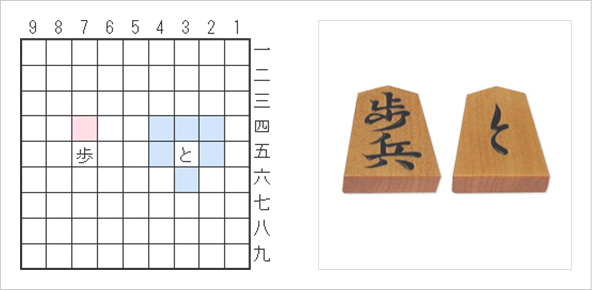
\includegraphics[keepaspectratio=true,width=\dimpx{400}]{../images/shogi_03_img_8}{}\mdline{19}%mdk

%mdk-data-line={21}
\mdline{21}(\mdline{21}\href{https://www.shogi.or.jp/knowledge/shogi/03.html}{日本将棋連盟公式サイト}\mdline{21}より転載)%mdk
%mdk
\end{mdframe}\label{section}%mdk%mdk

%mdk-data-line={23}
\begin{mdframe}%mdk

\frametitle{選択可能}\label{heading-section}%mdk%mdk

%mdk-data-line={24}
\noindent\mdline{24}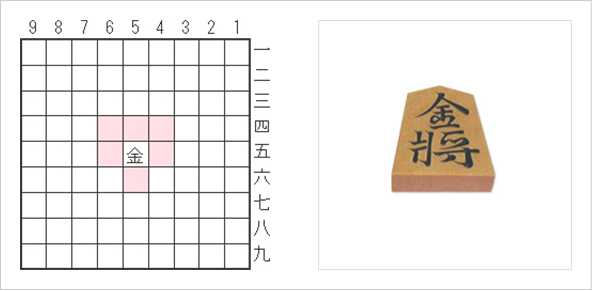
\includegraphics[keepaspectratio=true,width=\dimpx{400}]{../images/shogi_03_img_4}{}\mdline{24}
\mdline{25}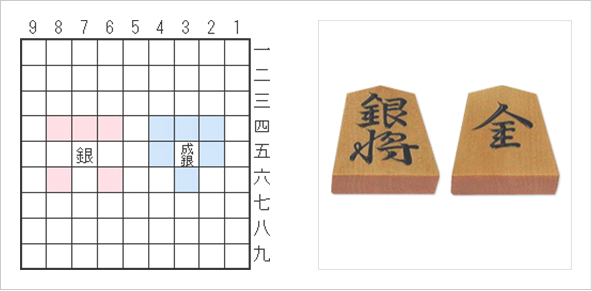
\includegraphics[keepaspectratio=true,width=\dimpx{400}]{../images/shogi_03_img_5}{}\mdline{25}
\mdline{26}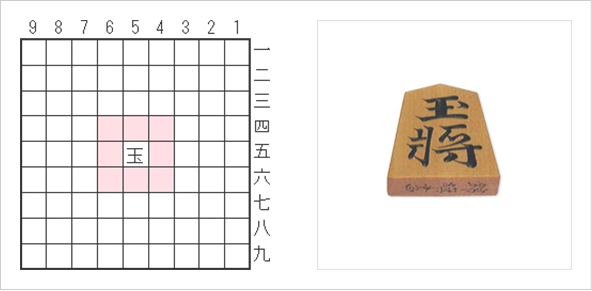
\includegraphics[keepaspectratio=true,width=\dimpx{400}]{../images/shogi_03_img_1}{}\mdline{26}%mdk

%mdk-data-line={28}
\mdline{28}(\mdline{28}\href{https://www.shogi.or.jp/knowledge/shogi/03.html}{日本将棋連盟公式サイト}\mdline{28}より転載)%mdk

%mdk-data-line={30}
\mdline{30}選択可能な動かし方を列挙していきたい%mdk
%mdk
\end{mdframe}\label{section}%mdk%mdk

%mdk-data-line={32}
\begin{mdframe}%mdk

\frametitle{選択可能を再帰的にすると}\label{heading-section}%mdk%mdk

%mdk-data-line={33}
\noindent\mdline{33}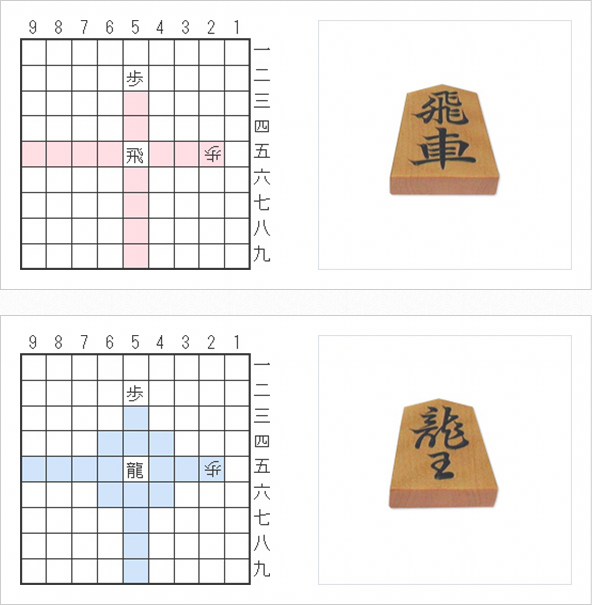
\includegraphics[keepaspectratio=true,width=\dimpx{400}]{../images/shogi_03_img_2}{}\mdline{33}
\mdline{34}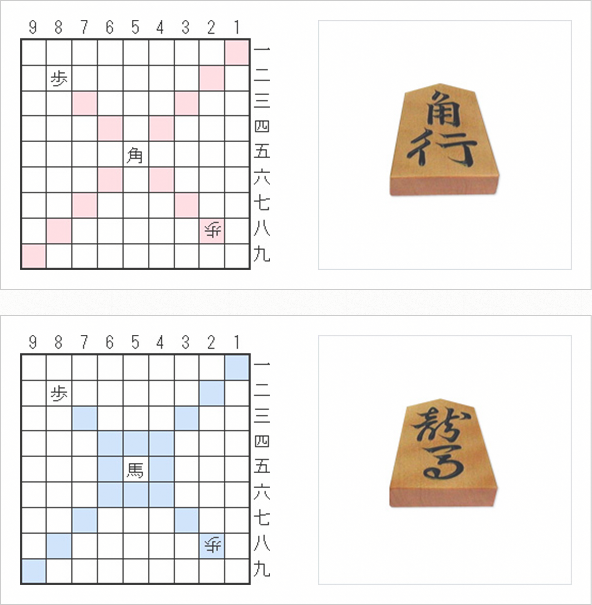
\includegraphics[keepaspectratio=true,width=\dimpx{400}]{../images/shogi_03_img_3}{}\mdline{34}
\mdline{35}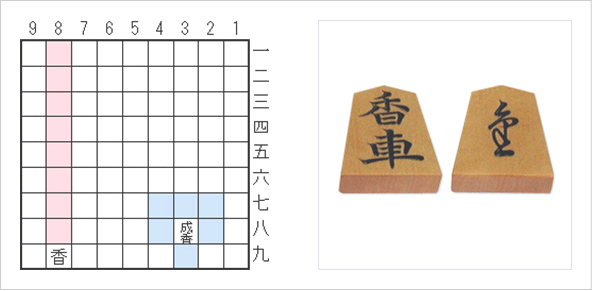
\includegraphics[keepaspectratio=true,width=\dimpx{400}]{../images/shogi_03_img_7}{}\mdline{35}
(\mdline{36}\href{https://www.shogi.or.jp/knowledge/shogi/03.html}{日本将棋連盟公式サイト}\mdline{36}より転載)%mdk
%mdk
\end{mdframe}\label{section}%mdk%mdk

%mdk-data-line={38}
\begin{mdframe}%mdk

\frametitle{選択可能を再帰的にすると}\label{heading-section}%mdk%mdk

%mdk-data-line={39}
\noindent\mdline{39}飛び道具 = 飛車、角、香車%mdk

%mdk-data-line={41}
\mdline{41}空白のマスに動かしたとき同じ動きを繰り返すか、そこで止まるかという選択可能性が与えられる%mdk
%mdk
\end{mdframe}\label{section}%mdk%mdk

%mdk-data-line={43}
\begin{mdframe}%mdk

\frametitle{参考:再帰的でないジャンプ}\label{heading-section}%mdk%mdk

%mdk-data-line={44}
\noindent\mdline{44}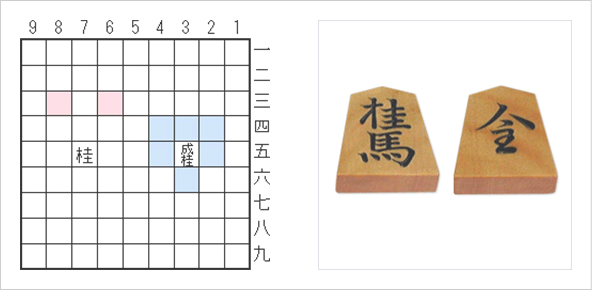
\includegraphics[keepaspectratio=true,width=\dimpx{400}]{../images/shogi_03_img_6}{}\mdline{44}%mdk

%mdk-data-line={46}
\mdline{46}(\mdline{46}\href{https://www.shogi.or.jp/knowledge/shogi/03.html}{日本将棋連盟公式サイト}\mdline{46}より転載)%mdk
%mdk
\end{mdframe}\label{section}%mdk%mdk

%mdk-data-line={57}
\begin{mdframe}%mdk

\frametitle{パーサーっぽい}\label{heading-section}%mdk%mdk

%mdk-data-line={58}
\noindent\mdline{58}香車 = \mdline{58}\mdcode{歩+}\mdline{58}%mdk

%mdk-data-line={60}
\mdline{60}\mdcode{香車~=~(【歩→空】【止】)~\textbar{}(【歩→空】【香車】)\textbar{}~(【歩→相手】【止】)}\mdline{60}%mdk

%mdk-data-line={62}
\mdline{62}\mdcode{--~【歩→自分】の場合は選択可能でない}\mdline{62}%mdk

%mdk-data-line={64}
\mdline{64}飛車や角、香車\mdline{64}\mdfootnote{1}{%mdk-data-line={106}
%mdk-data-line={106}
\noindent\mdline{106}いわゆる「飛び道具」%mdk
\label{fn-1}%mdk%mdk
}\mdline{64}は、相手の駒を取るとストップし、自分のコマは飛び越せない。%mdk
%mdk
\end{mdframe}\label{section}%mdk%mdk

%mdk-data-line={66}
\begin{mdframe}%mdk

\frametitle{例}\label{heading-section}%mdk%mdk

%mdk-data-line={67}
\noindent\mdline{67}【歩→空】【歩→空】【歩→空】【歩→空】【止】→ OK%mdk

%mdk-data-line={69}
\mdline{69}【歩→空】【歩→空】【歩→空】【歩→相手】【止】→ OK%mdk

%mdk-data-line={71}
\mdline{71}【歩→空】【歩→\mdline{71}\textbf{相手}\mdline{71}】【歩→空】【歩→空】【止】→\mdline{71}\textbf{NG}\mdline{71}%mdk

%mdk-data-line={73}
\mdline{73}【歩→空】【歩→空】【歩→空】【歩→\mdline{73}\textbf{自分}\mdline{73}】【止】→ \mdline{73}\textbf{NG}\mdline{73}%mdk
%mdk
\end{mdframe}\label{section}%mdk%mdk

%mdk-data-line={75}
\begin{mdframe}%mdk

\frametitle{駒モナド}\label{heading-section}%mdk%mdk

%mdk-data-line={76}
\noindent\mdline{76}Listモナドと状態モナド(State)を組み合わせた。%mdk

%mdk-data-line={78}
\mdline{78}あり得る動きをリストで表す%mdk

%mdk-data-line={80}
\mdline{80}駒を動かすと盤の状態が変更される%mdk
\begin{mdpre}%mdk
\noindent{\mdcolor{navy}type}~{\mdcolor{teal}PieceM}~{\mdcolor{teal}a}~{\mdcolor{navy}=}~{\mdcolor{teal}StateT}~{\mdcolor{teal}(}{\mdcolor{teal}(}{\mdcolor{teal}Int}{\mdcolor{teal},}~{\mdcolor{teal}Int}{\mdcolor{teal})}{\mdcolor{teal},}~{\mdcolor{teal}Field}{\mdcolor{teal})}~{\mdcolor{teal}{}[}{\mdcolor{teal}]}~{\mdcolor{teal}a}~{\mdcolor{darkgreen}--~駒モナド}\\
{\mdcolor{darkgreen}--~{}[]~は~リストのこと}\\
{\mdcolor{darkgreen}--~(Int,~Int)は駒の位置を表す}\\
{\mdcolor{darkgreen}--~((Int,~Int),~Field)~-\textgreater{}~{}[(((Int,~Int),~Field),~a)]}%mdk
\end{mdpre}%mdk
\end{mdframe}\label{section}%mdk%mdk

%mdk-data-line={90}
\begin{mdframe}%mdk

\frametitle{飛び道具}\label{heading-section}%mdk%mdk
\begin{mdpre}%mdk
\noindent moveAll~{\mdcolor{teal}::}~{\mdcolor{teal}PieceM}~{\mdcolor{teal}(}{\mdcolor{teal}Either}~{\mdcolor{teal}(}{\mdcolor{teal}Piece}{\mdcolor{teal},}~{\mdcolor{teal}(}{\mdcolor{teal}Int}{\mdcolor{teal},}~{\mdcolor{teal}Int}{\mdcolor{teal})}{\mdcolor{teal})}~{\mdcolor{teal}(}{\mdcolor{teal}Int}{\mdcolor{teal},}~{\mdcolor{teal}Int}{\mdcolor{teal})}{\mdcolor{teal})}~{\mdcolor{teal}-\textgreater{}}~{\mdcolor{teal}PieceM}~{\mdcolor{teal}(}{\mdcolor{teal}Int}{\mdcolor{teal},}~{\mdcolor{teal}Int}{\mdcolor{teal})}\\
{\mdcolor{darkgreen}--~Eitherは、駒を取ったかどうかを表す}\\
moveAll~move1~{\mdcolor{navy}=}~{\mdcolor{navy}do}\\
~~loc2~\textless{}-~move1~{\mdcolor{darkgreen}--~move1に歩を指定すると、`moveAll~歩`は香車の動きになる}\\
~~{\mdcolor{navy}case}~loc2~{\mdcolor{navy}of}\\
~~~~{\mdcolor{purple}Left}~(pie,~xy)~{\mdcolor{navy}-\textgreater{}}~{\mdcolor{navy}do}~{\mdcolor{darkgreen}--~相手の駒を取った場合、そこで止まる}\\
~~~~~~\_1~.=~xy\\
~~~~~~return~(xy{\mdcolor{teal}::}{\mdcolor{teal}(}{\mdcolor{teal}Int}{\mdcolor{teal},}~{\mdcolor{teal}Int}{\mdcolor{teal})})\\
~~~~{\mdcolor{purple}Right}~xy~{\mdcolor{navy}-\textgreater{}}~{\mdcolor{navy}do}~{\mdcolor{darkgreen}--~空白のマス目の場合再帰できる}\\
~~~~~~\_1~.=~xy\\
~~~~~~(moveAll~move1)~`mplus`~use~\_1~~{\mdcolor{darkgreen}--~もう一度動くか、止まるか~~選ぶ}%mdk
\end{mdpre}%mdk
\end{mdframe}\label{section}%mdk%mdk

%mdk-data-line={109}
\begin{mdframe}%mdk

\frametitle{和の演算:駒で足し算}\label{heading-section}%mdk%mdk

%mdk-data-line={110}
\noindent\mdline{110}竜や馬は「王または飛車、角」で表す。%mdk

%mdk-data-line={112}
\mdline{112}斜めを\mdline{112}\mdcode{縦\textgreater{}\textgreater{}横}\mdline{112}で表そうとしたが、それはダメだ%mdk
%mdk
\end{mdframe}\label{section}%mdk%mdk

%mdk-data-line={115}
\begin{mdframe}%mdk

\frametitle{課題}\label{heading-section}%mdk%mdk

%mdk-data-line={116}
\begin{itemize}[noitemsep,topsep=\mdcompacttopsep]%mdk

%mdk-data-line={116}
\item\mdline{116}将棋の駒を状態系モナドで表すのは、データ構造で表すのと違ってファイル出力などに向かない

%mdk-data-line={117}
\begin{itemize}[noitemsep,topsep=\mdcompacttopsep]%mdk

%mdk-data-line={117}
\item\mdline{117}状態モナドは関数なので%mdk
%mdk
\end{itemize}%mdk%mdk

%mdk-data-line={118}
\item\mdline{118}盤の境界を破ったときの処理が、盤の側のエラーはなくパースエラーしかない%mdk

%mdk-data-line={119}
\item\mdline{119}反則手を指すと盤が消える

%mdk-data-line={120}
\begin{itemize}[noitemsep,topsep=\mdcompacttopsep]%mdk

%mdk-data-line={120}
\item\mdline{120}複数盤に分岐している場合は反則のものが消えるのはいいが、盤が1つだけのときに消えるのは困る%mdk
%mdk
\end{itemize}%mdk%mdk
%mdk
\end{itemize}%mdk
%mdk
\end{mdframe}\label{section}%mdk%mdk

%mdk-data-line={122}
\begin{mdframe}%mdk

\frametitle{今後の新機能候補}\label{heading-section}%mdk%mdk

%mdk-data-line={123}
\begin{itemize}[noitemsep,topsep=\mdcompacttopsep]%mdk

%mdk-data-line={123}
\item\mdline{123}王手・詰み判定%mdk

%mdk-data-line={124}
\item\mdline{124}量子将棋%mdk

%mdk-data-line={125}
\item\mdline{125}中将棋

%mdk-data-line={126}
\begin{itemize}[noitemsep,topsep=\mdcompacttopsep]%mdk

%mdk-data-line={126}
\item\mdline{126}獅子%mdk
%mdk
\end{itemize}%mdk%mdk

%mdk-data-line={127}
\item\mdline{127}棋譜の読み込み/書き出し%mdk
%mdk
\end{itemize}%mdk
%mdk
\end{mdframe}\label{section}%mdk%mdk%mdk%mdk%mdk


\end{document}
